\documentclass[conference, compsocconf, letterpaper]{IEEEtran}

\usepackage[utf8]{inputenc} % set input encoding (not needed with XeLaTeX)

%%% PAGE DIMENSIONS
%\usepackage{geometry} % to change the page dimensions
%\geometry{a4paper} % or letterpaper (US) or a5paper or....
% \geometry{margins=2in} % for example, change the margins to 2 inches all round
% \geometry{landscape} % set up the page for landscape
%   read geometry.pdf for detailed page layout information

\usepackage{graphicx} % support the \includegraphics command and options

% \usepackage[parfill]{parskip} % Activate to begin paragraphs with an empty line rather than an indent

%%% PACKAGES
\usepackage{booktabs} % for much better looking tables
\usepackage{array} % for better arrays (eg matrices) in maths
\usepackage{paralist} % very flexible & customisable lists (eg. enumerate/itemize, etc.)
\usepackage{verbatim} % adds environment for commenting out blocks of text & for better verbatim
\usepackage{subfig} % make it possible to include more than one captioned figure/table in a single float
% These packages are all incorporated in the memoir class to one degree or another...
\usepackage{algorithm}
\usepackage{algpseudocode}
\usepackage{amsthm}


%%% HEADERS & FOOTERS
\usepackage{fancyhdr} % This should be set AFTER setting up the page geometry
\pagestyle{fancy} % options: empty , plain , fancy
\renewcommand{\headrulewidth}{0pt} % customise the layout...
\lhead{}\chead{}\rhead{}
\lfoot{}\cfoot{\thepage}\rfoot{}

%%% SECTION TITLE APPEARANCE
%\usepackage{sectsty}
%\allsectionsfont{\sffamily\mdseries\upshape} % (See the fntguide.pdf for font help)
% (This matches ConTeXt defaults)

%%% ToC (table of contents) APPEARANCE
%\usepackage[nottoc,notlof,notlot]{tocbibind} % Put the bibliography in the ToC
%\usepackage[titles,subfigure]{tocloft} % Alter the style of the Table of Contents
%\renewcommand{\cftsecfont}{\rmfamily\mdseries\upshape}
%\renewcommand{\cftsecpagefont}{\rmfamily\mdseries\upshape} % No bold!

%%% END Article customizations

%%% The "real" document content comes below...

\title{Using Chord as a Platform for Software as a Service for a Generalized, Distributed MapReduce.}
\author{
Andrew Rosen \qquad Brendan Benshoof \qquad Matt Erwin \qquad Anu Bourgeois  \\Department of Computer Science, Georgia State University\\ 34 Peachtree St NW \\ Atlanta, Georgia 30303\\  rosen@cs.gsu.edu }
%\date{} % Activate to display a given date or no date (if empty),
         % otherwise the current date is printed 

\begin{document}
\maketitle

\begin{abstract}
DRAFT ABSTRACT:  We developed a Peer-to-peer architecture for software as a service. We show viability by implementing MapReduce.
MapReduce does not automatically distribute work among slave nodes without configuration.  In Chord, nodes are evenly distributed and  are responsible for files based on their position in the network. We exploit this property to automatically distribute MapReduce tasks evenly among nodes in the same manner. 
\end{abstract}


\section{Introduction}


Peer-to-peer (P2P) networks are of enormous interest to network research, as they provide an efficient way to distribute large files to millions of users without many of the limitations of the traditional client-server model. In the client-server model, the server addresses each client's request individually, creating a single point of failure due to traffic or the loss of the server.  In peer-to-peer networks, each node takes on both the role of client and server.  If someone wishes to introduce data into the a peer-to-peer network, peers can both request the file and distribute it to others.  This takes much of the burden of file distribution off of what would have normally been an extremely busy server \cite{Overview}.  

P2P networks have resulted in an unprecedented amount of data being purveyed through the Internet.  While recent studies show that P2P accounts for 13.2\% of downstream traffic, down from its peak of 40\% of all Internet traffic, the actual volume of P2P traffic is at its highest yet \cite{5713296}. Many companies have embraced legal uses of P2P technology, such as providing ways to stream media or provide large updates  \cite{P2PLegal}.  For example, Blizzard uses a modified BitTorrent protocol to distribute updates and patches to millions of users for games such as World of Warcraft and Starcraft II \cite{chehai2006analysis}.



\subsubsection{SaaS}
In recent years, there has been a trend of crowdsourcing large and complicated tasks among willing participants.  

Folding@home \cite{folding}. 

seti at home that kind f thing



Our thing is totally way better because it we're making it generic, knatch.  Why is generic better?  becuase it makes it easier for developers. 

We create the system and genericized version of map-reduce 

\subsubsection{Current models of distributing work}




\section{Background}
Not all peer-to-peer networks are equal; there are variety of protocols and methodologies that a networks could implement and this affects what kind of solutions are available to reduce the traffic on the network    \cite{SurveyCompare} \cite{Overview}.

%\subsection{Basic Peer-to-Peer Networks}
The most basic type of network is a structured, centralized  network.  Peers in this network communicate with a central server to provide their files and to locate other peers that have the files they are searching for.  This is structured in the sense that the layout of the overlay network is tightly controlled, in this case by the server(s). While this avoids the problems of routing, it has the same issues of scalability as a client-server layout and is not much of an improvement. An example of this network is the long defunct Napster  \cite{SurveyCompare} \cite{Overview}.

On the other side of the spectrum, there are unstructured, decentralized networks.  These networks create overlay links between nodes in a random manner. This leads to a very unstructured overlay, but it is one that is very easily constructed.  No single node is responsible for the whole of the network;  files are located by sending out requests to neighboring peers, which in turn request from their neighbors and so on. Should a file become suddenly popular, this flood of this requests can easily bring some peers to their knees, unable to deal with the high level of traffic \cite{Lv:2002:SRU:514191.514206}.  This makes these types of networks also a poor choice for implementation \cite{Overview}.

Modern P2P implementations are hard to classify easily, due to the variety of methods used to create a working network that avoids the weaknesses of the two above network types.  Many networks today use a decentralized structured approach to distribute files, where the topology of the overlay is constructed and controlled by the protocol and the information about the network is distributed among the peers.  This distribution is typically accomplished by a distributed hash table (DHT).  Networks that use a DHT choose specific peers in which to place information about how to find particular files or data.  These peers are chosen so that the peer's ID in the network corresponds to the file or data's ID, typically by hashing both ID's and comparing them  \cite{SurveyCompare}. 

In addition, the network topology is distributed among various peers.  Each peer has a table consisting of other peers in the network and the means of communicating with them.  The contents of this table are also controlled by the protocol.  The table handles the routing of requests from one node to another; when a peer receives a request it cannot fulfill, such as information about where to find a particular file, it directs the the request to the node that is "closest" to the destination of the request. How this works is determined by each protocol \cite{Chord}.  It should be noted that closeness is relative to the algorithm; depending on what identifiers are assigned, a node in New York City might be "close" to a node in Russia, but "far" from a node physically a few miles away.  Examples of protocols that use these techniques are trackerless BitTorrent \cite{BitTorrent}, Chord \cite{Chord}, and Kademlia \cite{Kademlia}. As our work is implemented using Chord, we provide more detail in the following section. 


\subsection{Related Work}

The Cooperative File System (CFS) is a file sharing system built on top of Chord \cite{CFS} which extended the idea of storing files to storing chunks of files. 

P2P-MapReduce \cite{marozzo2012p2p}, is similar to our work, but looks only at MapReduce; MapRecude is only one of the services CHRONUS provides.  It consumed more network resources than the traditional centralized implementation, but was much more tolerant to churn and lost less time when nodes?jobs failed\footnote{Fix this, actual quote was "In summary, the experimental results show that even if the P2P-MapReduce system consumes in most cases more network resources than a centralized implementation of MapReduce, it is far more efficient in job management since it minimizes the lost computing time due to jobs failures."}.  P2P-MapReduce was not implemented on a large scale; the test results for larger networks were derived from simulations

\subsubsection{Folding at home?}
Folding@home \cite{folding}

\section{CHORD}
The Chord protocol \cite{Chord} takes in some key and returns the identity (ID) of the node responsible for that key.  These keys are generated by hashing a value of the node, such as the IP address, or by hashing  the filename of a file.  The hashing process creates a $m$-bit hash identifier.

The nodes are then arranged in a ring from the lowest hash-value to highest.  Chord then takes the hashed files and places each in the node that has the same hashed identifier as it.  If no such node exists, the node with the first identifier that follows this value.  This node responsible for the key $\kappa$ is called the $successor$ of $\kappa$, or $successor(\kappa)$.  Since we are dealing with a circle, this assignment is done in module $2^m$ space.  For example, if there were some portion of the network with nodes 20, 25, and 27, node 25 could be responsible for the files with the keys (21,22,23,24,25). If node 25 were to decide to leave the network, it would inform node 27, who would then be responsible for all the keys node 25 was covering. An example Chord network is drawn in in Figure \ref{chordreal}.

With this scheme, we can reliably find the node responsible for some key by asking the next node in the circle for the information, who would then pass the request through the circle until the successor was found.  We can then proceed to directly connect with the successor to retrieve the file.  This naive approach is largely inefficient, and is a simplification of the lookup process, but it is the basis of how Chord theoretically works.

To speed up the lookup time, each node builds and maintains a \emph{finger table}.  The \emph{finger table} contains the locations of up to $m$ other nodes in the ring.  The $i$th entry of node $n$'s \emph{finger table} corresponds to the node that is the $successor(n+2^{i-1})$ $mod$ $2^m$ \footnote{Because hash values won't be perfectly distributed, it is perfectly acceptable to have duplicate entries in the \emph{finger table}.}. 


\subsection{Stabilize} 

When a node $n$ is told to find some key, $n$ looks to see if the key is between $n$ and $successor(n)$ and return $successor(n)$'s information to the requester. If not, it looks for the entry in the finger table for the closest preceding node $n'$ it knows and asks $n'$ to find the successor.  This allows each step in the to skip up to half the nodes in the network, giving a $\log_2(n)$ lookup time.  Because nodes can constantly join and leave the network, each entry in the table is periodically checked and updated. 

To join the network, node $n$ first asks $n'$ to find $successor(n)$ for it.  ,but those nodes won't  acknowledge $n$'s presence in the ring yet\footnote{This is fine. You don't have to be \emph{in} the ring to interact with it.  You just have to be able to talk to a node in the ring.}.  Node $n$ relies on the stabilize routine to fully integrate into the ring.

The stabilize routine helps the network adjust to churn. Each node periodically checks to see who their successor's predecessor is.  In the case of a static network, this would be the checking node.  However, if the checking node gets back a different node, it looks at that returned node's hash value and changes their successor if needed.  Regardless of whether the checking node changes its successor, that node then notifies the ( possibly) new successor,  essentially telling the successor "based on the information I have, I'm your predecessor.  Check to see if you need to update your predecessor information," to which the successor obliges.  A more concrete example:


Suppose Alice, Bob, Carol, and Dan are members of the ring and everyone happens to be ordered alphabetically (Figure \ref{abcd1}). Alice is quite sure that Carol is her successor.  Alice asks Carol who her predecessor is and Carol says Bob is.  Since Bob is closer than Carol, Alice changes her successor to Bob and notifies him.  

When Bob sees that notification, he can see Alice is closer than whoever his previous predecessor is and sets Alice to be his predecessor.  During the next stabilization cycle, Alice will see that she is still Bob's predecessor and notify him that she's still there (Figure \ref{abcd2}).

\begin{figure}
    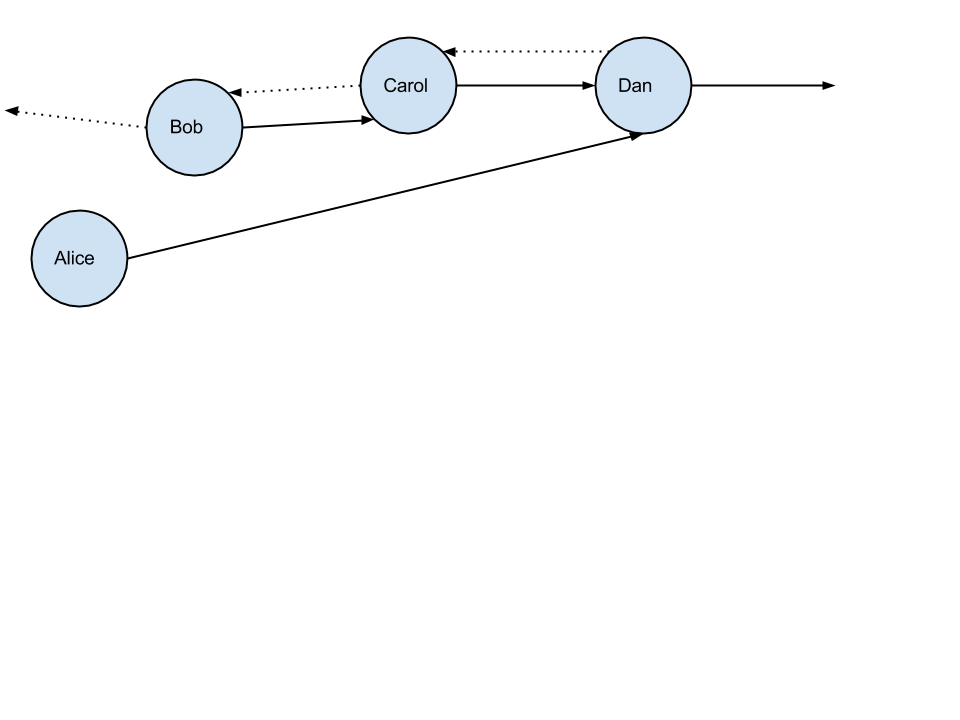
\includegraphics[width=\linewidth]{abcd1}
    \caption{Alice has incorrectly determined that Carol is her appropriate successor.  When Alice stabilizes, Carol will let her know about Bob.}
    \label{abcd1}
\end{figure}


\begin{figure}
    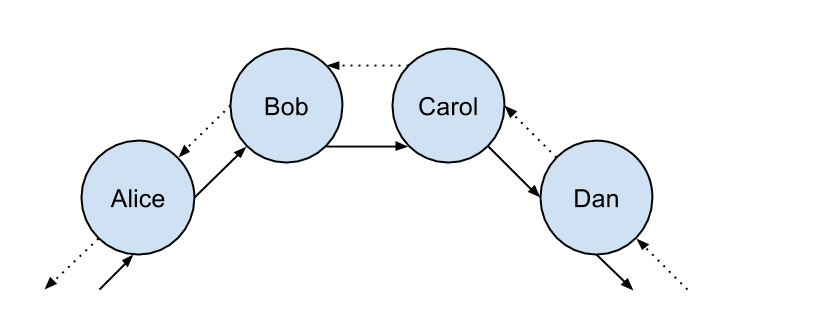
\includegraphics[width=\linewidth]{abcd2}
    \caption{After completing stabilize, Alice makes Bob her successor and notifies him. Bob then made Alice as his predecessor.}
    \label{abcd2}
\end{figure}



\subsubsection{Responsibility}
One of the major design choices for Chord implementation is not figuring which node is responsible for a given key, but figuring out who decides which node is responsible for a given key.


In our implementation, a node $n$ is responsible for the keys ($predecessor(n)$, $n$].  In other words, when $n$ gets a message, it considers itself the intended destination for the message if the message's destination hash is between $predecessor(n)$ and $n$.  A node that does not have a predecessor assigns itself as its own predecessor and considers itself responsible for all messages it receives.  COUNTER WHY THIS IS A BAD IDEA.  THIS IS A VERY DEFINITE CRITICISM 


\subsubsection{reassigning responsibility}
When a node discovers that he is no longer responsible for certain things, this is what happens

\subsubsection{hanlding churn and politely quitting}
Due to the potentially volatile nature of a peer-to-peer network, Chord has to be able to handle (or at the very least, tolerate) an arbitrary amount of churn.  We've already detailed how Chord gradually guides nodes into their correct locations after they join the network.  The same is true for when a node leaves the network; the stabilize procedure will guide nodes to their correct successors and predecessors.  However, we can exert more control over how to handle nodes leaving the network

A node can leave the ring in one of two ways.  A node can either suddenly drop out of existence, or a node can tell the network he is about to leave, letting his successor and predecessor immediately perform the needed changes.  

\subsubsection{the general idea of backup}
Unfortunately, it is impossible that every time a node leave the network it will do so politely.  If a node suddenly quits, the data it had stored goes with it. To prevent data from becoming irretrievable, a node can periodically send backups to its successor.  So as not to overwhelm the ring with a cascade of backups of backups, the node only passes along what it considers itself responsible for, which can change .

This process does not cascade, as nodes will only backup things it is responsible for.


\subsubsection{}
\section{MapReduce}
At its core, MapReduce \cite{mapreduce} is a system for division of labor.  A task gets sent to a master node, who then divides that task among slave nodes, which may further divide the task.  This task has two distinct parts: Map and Reduce.  Map performs some operation on a set of data and then reduces a result for each map operation.  This intermediate data is then reduced by other slave nodes then returned to the user. 

\subsection{Summary}

Summary of MapReduce \cite{mapreduce} 

Hadoop is this an open source thingy for MapReduce \cite{hadoop}

\subsection{Map}
\subsection{Reduce}


\section{CHRONUS}




\subsection{Implementation}
Parapgraph here about the bidding nature of the amazon market.
age of the inherent ring structure.





\subsubsection{Code Details}
We implemented the Chord based on the psuedocode  in the Stoica's paper \cite{Chord}, using Python instead of C++.  We also sent messages instead of performing remote procedure calls.


\subsubsection{chunking and mechanics }

Dabek CFS \cite{CFS}

Design choice of CFS and replication 


Rather than storing the whole file in the appropriate node, we instead split the file into arbitrary-sized chunks of data.  Each of the chunks are then hashed and sent to their corresponding node.

\subsubsection{backup implementation and mechanics}
Paragraph about backup

\subsubsection{Issues of normal MapReduce } 




\subsection{Distributed MapReduce}
To do a fully distributed map reduce, each node takes on responsibilities of both a slave and master, much in the same way that a node in a p2p file-sharing service will act as both a client and a server.   
\subsubsection{Recap the issues  of normal MapReduce  and why ours is bettter} 


\subsubsection{Writing your own MapReduce}
The big advantage of our system is the ease of development.  All a developer needs to do to write three functions: the staging function, map, and reduce.  The staging function splits the work into \emph{data atoms}, which are the smallest individual units that work can be done on.  This might a line of text in a document, OR OTHER EXAMPLES

The map function works as a user would expect, running a function over a series of values and outputing a list of intermediate \emph{data atoms}.  Reduce takes in two \emph{data atoms} and combines them into one.

The developer does not need to worry about distributing work evenly, nor does he have to worry about any node in the network going down.  The underlying Chord ring handles that automatically.


Sample code can be found in FIGURE SOME NUMBER



\subsubsection{Running Map Reduce}
\subsubsection{Redundancy of the "Master" Node}
We don't have a master node, we have a stager.  If he goes down, everything ends up in his successor



\subsubsection{Redundancy of the Slave nodes}
We backup our jobs and remove the backups as we're going

\subsubsection{How do we know when we're done}


\subsection{In which we address possible criticism}
\subsubsection{The issue with chunking and IRM}
Mutually incomparable

\subsubsection{If we hash a filename to get the identifier, then you can't have two same file names.}
\subsubsection{Determining when you're done is expensive}
As a whole yes, but merging two sorted lists is $O(n)$ time.  A distributed merge sort is $O( \frac{n \cdot \log (n)}{m} $ time????? CITATION NEEDED, where $m$ is 


\subsubsection{Disjoint rings}

\subsubsection{The security we didn't do}
We can have multiple non interacting secure file systems.


\section{Experiments}
A set of experiments were run on large groups of Amazon EC2 Micro Instances\cite{amazon-micro}.
\section{Results}

\section{Conclusion}
Our stuff \cite{code} is awesome.

\bibliographystyle{plain}
\bibliography{CHRONUS}
\end{document}
